\documentclass[12pt]{article}
\usepackage[utf8]{inputenc}
\usepackage{graphicx}
\usepackage[table]{xcolor}
\usepackage{longtable}
\usepackage{layout}
\usepackage[a4paper,width=150mm,top=25mm,bottom=25mm]{geometry}
\usepackage[style=apa,sorting=nyt]{biblatex}
\addbibresource{bib.bib}
\usepackage{float}
\graphicspath{/images}
\usepackage{array}
\graphicspath{{images/}}
\usepackage{lscape}
\title{
    
    {Stage 3 PhD Proposal}\\
    {Understanding and Predicting Well-being Trajectory Through Proxy Data Streams}\\
    {\large University of Nottingham}\\
    {\large Horizon Centre for Doctoral Training}\\
}
\author{Gregor Milligan}
\date{June 2022}

\begin{document}
\maketitle
\section*{Supervisors}
James Goulding\\
Liz Dowthwaite

\tableofcontents
\clearpage
\section{Introduction and Problem Statement}

Well-being is a multidimensional construct and the state of an individual’s well-being is ever shifting; this changing state of well-being is difficult to measure and predict. There are numerous tools and techniques that can be used to understand the current state of an individual’s well-being \parencite{clarke_warwick-edinburgh_2011, diener_new_2010, watermanQuestionnaireEudaimonicWellBeing2010}; however, predicting well-being temporally using traditional well-being measures is a challenge. The overarching goal of this project is to examine proxy lenses which could support the understanding and prediction of well-being at scale. 

Proxy lenses, such as less frequently used or novel data sources, may be utilised to understand and predict well-being. A source of interest is social media data as it has previously been used to accurately gauge the subjective well-being of individuals and broader populations \parencite{jaidka_estimating_2020}. Social media data can provide a further temporal understanding and finer granularity to different well-being facets, emotional well-being or satisfaction with life, through the exploration of language analysis and platform interaction behaviour \parencite{luhmann_using_2017}. Other data streams that could be used to understand well-being include socioeconomic indicators of populations and health data (Electronic Health Records). These data sources have been suggested as an alternative or complement to traditional well-being measures when understanding well-being over time \parencite{voukelatou_measuring_2021}.
 
Predicting well-being trajectory through proxy data streams could facilitate a more nuanced understanding of well-being across the United Kingdom, which could aid in informing well-being related policy and understanding the co-occurring health impacts of well-being. This is a challenging time as society is facing a financial and political crisis and instability, policymakers could integrate well-being insight into policy development to prevent deleterious societal effects \parencite{voukelatou_measuring_2021}. In the context of digital mental health platforms, well-being evaluation could facilitate a system that enables self-reflection and well-being pathways to support practitioners and users within platforms. Overall, this research aims to define the unique applications and challenges of using novel data sources to evaluate and predict well-being trajectories.

\subsection{Industry Partner and Other Digital Mental Health Platforms}
Kooth is a digital counselling and support platform split into two services: “Kooth”, a service platform for children and young people (CYP) aged between 11-25 years old, and “Qwell”, a service for adults aged over 18 years old (Hanley et al., 2021). Kooth and Qwell give both adults, and young people access to a community formed around mental health. The platforms are made up of four key elements: a chat service, enabling users to open a dialogue with a team of professionals about their mental health concerns. A message board/forum allows users to interact with other users through discussion boards, articles created by both staff and users, and a private journal. Only data from users who have consented to have their data used for research purposes will be accessed.

The different elements of the Kooth platforms will continue to generate a large amount of data; usage data is generated when users access the platforms, for example, the number of times a user accessed a particular part of the site. Other data consists of text data from interactions with practitioners, user diary entries and interactions on discussion boards.

It would be valuable to explore how other platforms related to mental health and well-being could offer insight into the prediction of well-being; alternative digital mental health interventions such as WYSA provide services comparable to Kooth such as self-care tools and therapist support, WYSA also uses an artificial intelligence-based chatbot that users can interact with \parencite{inkster_empathy-driven_2018}; the platform Headspace provides “Mindfulness Interventions” rather than a specific mental health intervention \parencite{zollars_effects_2019}. Data generated on alternative platforms could offer unique insights to evaluate well-being, although gaining access to data generated on alternative platforms may not be possible or present significant challenges.  


\section{Research Questions and Objectives}
The overarching goal of this PhD is to understand how proxy data streams can be used to understand and predict well-being and the broader impact that this understanding could bring to digital mental health platform service delivery.\\
\begin{enumerate}
    \item How can data-driven methods be used to understand well-being trajectory at scale?\\
    Objectives to answer question 1:
     \subitem  a) Explore what data-driven techniques and proxy data sources are appropriate for understanding and predicting well-being
    \subitem b)	Pinpoint the current challenges and viable solutions to quantifying and predicting well-being through proxy data streams
    \subitem c)	Understand how different well-being philosophies and frameworks can be used to inform data-driven model development
    \item How can outputs from data-driven models provide value to various stakeholders involved in the design, provision, or use of digital mental health platforms? \\ 
    Objectives to answer question 2:
    \subitem d)	Understand how well-being trajectories can be used to support individual self-reflection and mental health/well-being pathways
    \subitem e) Understand how well-being trajectory predictions can be used to assist practitioners of digital mental health platforms 

\end{enumerate}
\clearpage
\section{Methodology}
There will be a range of methodological approaches applied to this PhD due to the various tools and techniques used in the disciplines of computer science and psychology. Appendix A depicts a timeline of planned activities to answer the research questions, the first year will consist of a range of research projects that will enable a more detailed understanding of the potential impacts of the research. The initial set of studies will consist of landscape mapping, understanding the various stakeholders within digital mental health platforms, the data digital mental health platforms can provide, and the wider potential impact and applications of predicting well-being. The focus will then shift onto defining and predicting well-being through data-driven methods, exploring what tools and techniques are the most appropriate for predicting well-being while also exploring what different data sources could be used as proxy lenses to understand well-being. Then delving into the initial research gap, exploring how data from digital mental health platforms can contribute to understanding and predicting well-being, which has not yet been explored in the current literature.\\

Proposed Methodology to Answer Question 1:
This question will require the integration of different data-driven, machine learning and natural language processing techniques with data from different data sources to quantify and predict well-being. This enables an exploration of the applications of different data-driven methods, and the affordances both data-driven techniques and different data sources can provide when attempting to understand well-being. Furthermore, exposing the biases and challenges presented to researchers when attempting to quantify and predict psychological states, contributing to the completion of objectives A and B.

To complete objective C, an analysis of well-being measures will be undertaken to explore the way in which well-being frameworks, for example, the eudemonic activity model (Martela and Sheldon 2019), can be used as a framework to develop approaches for understanding well-being through proxy data streams and provide insight into behavioural or language patterns that may reveal well-being information. An exploration of how the eudemonic activity model and other eudemonic representations of well-being can be used to understand and predict well-being will be explored. This gap is suggested in the current preliminary literature review (Section 4.5).\\

Proposed Methodology to Answer Question 2:
This question will require a combination of qualitative and quantitative methodologies to understand the impact of well-being prediction fully. Techniques consisting of focus groups, interviews and surveys will be applied to scope out the current sentiment towards how well-being is expressed online and the stigma associated with well-being; also investigating the various stakeholders involved in the design, provision, or use of digital mental health platforms. From these initial investigations, the potential impact can be defined, therefore setting the groundwork for reflection of the output from data-driven models have been designed and implemented.


\section{Literature Review}
The overarching goal of this thesis is to examine proxy lenses through which well-being can be understood and predicted at scale. This review will consist of an overview of well-being and the different philosophical approaches; and the variety of tools and techniques used in psychology to understand well-being. This synthesis of well-being and well-being instruments will elucidate the various use-cases and pitfalls associated with said instruments. This foundational understanding of well-being will enable the exploration of the data-driven techniques currently being used to predict well-being and the data sources employed therein. Concluding with the remunerations, biases and difficulties of predicting well-being, using these datasets as different lenses to understand well-being; and the potential applications of the predictive outputs could be. 
\subsection{Defining Well-being}

Well-being can be defined as ideal psychological experience and functioning \parencite{ryan_happiness_2001}. Two prominent philosophies of well-being have been established; hedonistic (subjective) well-being \parencite{dienerSubjectiveWellbeing1984} and eudemonic well-being (EWB) \parencite{watermanTwoConceptionsHappiness1993}; each approach is based on fundamentally differing views of human nature.

The hedonic approach to well-being equates the well-being of an individual to the level of happiness or pleasure they experience. Diener (1984) clarifies the three contributing factors of subjective well-being (SWB): overall life satisfaction (LS); a high positive affect, emotions such as excitement, contentment, or interest; and low negative affect: emotions such as distress, guilt or fear.

The eudemonic approach to well-being is defined as to what degree people can be their most authentic self, with more nuance than just happiness and LS, but well-being also is related to actualising one’s individual potential \parencite{watermanTwoConceptionsHappiness1993}. Furthermore, \textcite{martela_clarifying_2019} express the idea that not all outcomes that produce pleasure are congruent with well-being; that well-being should be a combination of not only how a subject is feeling but why the subject feels a certain way and what the subject is doing to feel that way. \textcite{waterman_reconsidering_2008} presents the view that both approaches are interrelated but provide distinguishable nuance when conceptualising well-being. 

\textcite{martela_clarifying_2019} present the eudemonic activity model (EAM) [figure \ref{EAM}] as “a common core for connecting eudemonic and subjective well-being”. This tripartite approach to well-being is based on the self determination theory (SDT) assertion that all people share the evolved need for autonomy, competency, and relatedness \parencite{ryan_happiness_2001}. This model originated from the difficulty of comparing EWB studies due to the diverse range of EWB measurement strategies. “Doing well” and “Feeling well” are the two pillars of the EAM; “doing well” is derived from the eudemonic concept of the motivations and activities that enable and ultimately lead to self-realisation and the pursuit of excellence, of which the latter is an ever-shifting horizon. “Feeling well” can be divided further into two sections: Psychological need-satisfaction and SWB, with concepts including feelings of autonomy, competence, and relatedness, i.e. SDT and their causal link to the constructs in the SWB, i.e. life satisfaction \parencite{forgas_understanding_2018}. The EAM can be used as a framework to understand the interrelated intricacies of both philosophies.

\begin{figure}[H]
    \centering
    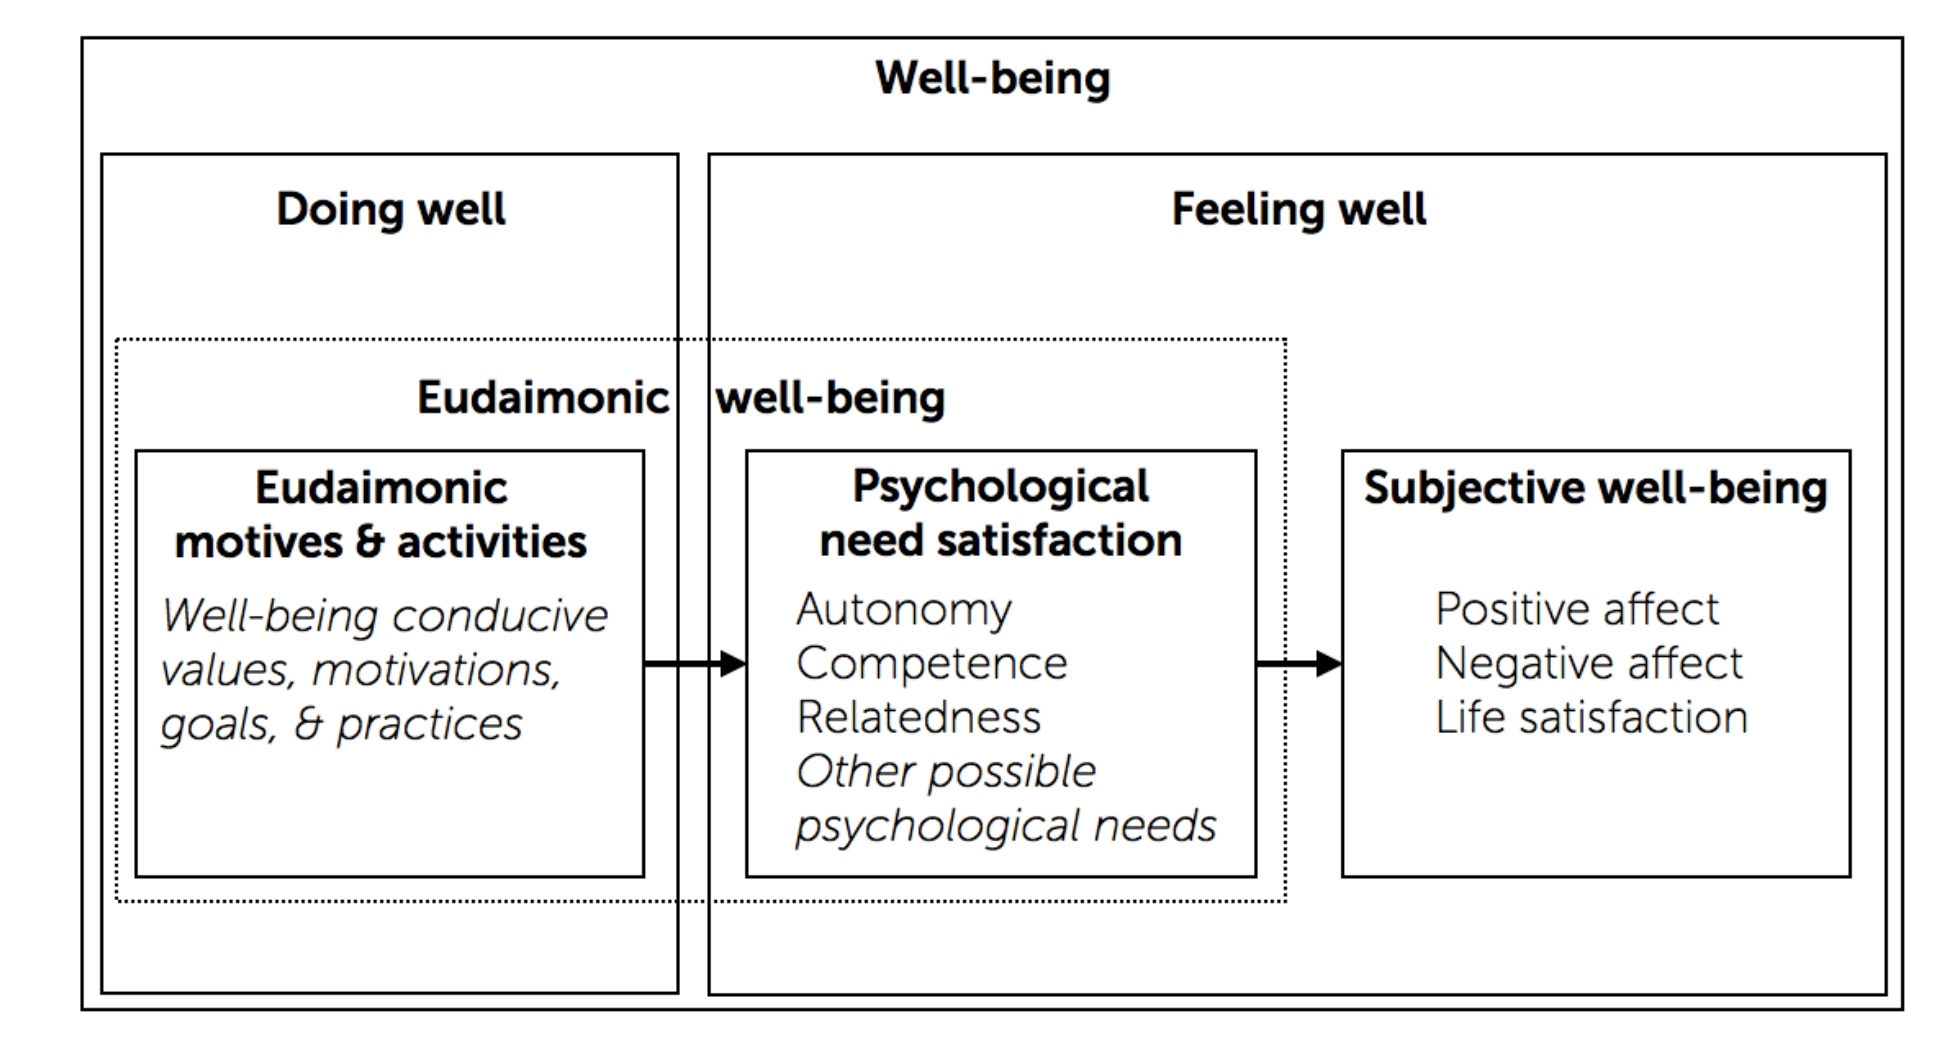
\includegraphics[width=0.85\textwidth]{Images/EAM.png}
    \caption{The eudaimonic activity model and the distinction between doing well and feeling well}
    \label{EAM}
\end{figure}

\subsection{Self-reported Well-being Instruments}
Standardised well-being instruments are used to assess and evaluate the well-being of individuals or populations. The most common approach for assessing well-being is that of self-reported well-being instruments, which regularly come with considerable scepticism regarding the interpretation and validity of self-reported data \parencite{Sandvik2009}. This scepticism stems from the pressure of an individual to conform to the societal expectation of happiness; it is worthwhile noting that this pressure to conform is also apparent in nonself-reported measures such as interviews \parencite{diener_response_1991}. \textcite{kozma_social_1988} suggested that social desirability is a substantive feature of an individual’s personality, closely linked to an individual’s SWB and therefore should not be considered a source of error when evaluating well-being. The multitude of well-being instruments available to researchers exemplifies the value that can be gleaned from even the most delicate gradations of well-being.
 
The applications for self-reported well-being instruments vary depending on the outcome measure of interest. The Warwick-Edinburgh Mental Well-being Scale (WEMWBS), and its short variant, the Short Warwick-Edinburgh Mental Well-being Scale (SWEMWBS), is a well-being instrument which measures the subjective well-being and functioning of the respondent \parencite{clarke_warwick-edinburgh_2011}. The Scale of Positive and Negative Experience (SPANE) is used to evaluate subjective well-being, specifically the range of positive and negative experiences a respondent faces and the balance of these experiences \parencite{diener_new_2010}. The Questionnaire for Eudaimonic Well-Being (QEWB) is a questionnaire that can be used to measure well-being in practice consistent with the eudemonist philosophy. QEWB is used to understand a respondent’s general level of eudemonic functioning, such as the pursuit of excellence and self-realisation \parencite{watermanQuestionnaireEudaimonicWellBeing2010}.

Other well-being measures include the Young Person’s Clinical Outcomes in Routine Evaluation (YP-CORE), designed for use in school counselling settings, focusing on generalisable functional and well-being issues \parencite{twigg_young_2009}; and the Strengths and Difficulties Questionnaire (SDQ) assessment tool, used internationally in clinical and community environments \parencite{goodman_strengths_1997}.

\textcite{mindel_assessing_2021} evaluated the suitability of SWEMWS, YP-CORE and SDQ in the context of a digital mental health platform for users aged 11- 15. A stratified random sampling method was undertaken to distribute assessment measures to a sample of users that primarily represented the Kooth user base. Based on the judgment of Kooth practitioners, all three measures demonstrated validity when used as indicators of user-rated needs upon entry to the Kooth platform, YP-CORE being the more appropriate measure in this context as it can be used to measure both user needs and outcomes. Mental health and well-being needs are unique for each service user, with young people wanting to be viewed as individuals \parencite{jacob_measuring_2017, sefi_testing_2021}. A better understanding of service users’ needs and the impact of outcomes would be improved by combining standardised measures with a tailored assessment of the individual \parencite{mindel_assessing_2021}. Applying natural language processing techniques to data generated on digital mental health platforms could provide part of a tailored assessment for individual users and provide insight that could aid in individual self-reflection or assist practitioners. 
\subsection{Data Driven Methods for Text}
Data-driven methods for text data involve the application of machine learning (ML) or statistical modelling techniques to identify relationships between the linguistic features contained in text. NLP methods are used to extract language features, which are then used to predict content using supervised or unsupervised machine learning techniques \parencite{jaidka_estimating_2020}. 
\textcite{shatte_machine_2018} conducted a scoping literature review of the applications of ML and big data in mental health, finding the use of NLP techniques on unstructured text data as a novel approach. Examples of NLP use-cases in the context of mental health are recognising schizophrenia in a corpus, detecting suicide ideation from counselling transcripts, and analysing social media data to detect depressive symptoms \parencite{strous_automated_2009, oseguera_automatic_2017, coppersmith_natural_2018}. The most common techniques for extracting mental health and well-being insight from text include sentiment analysis, topic modelling, text summarisation and keyword extraction \parencite{shatte_machine_2018}. 
\subsection{Natural Language Processing Overview}
Natural language processing (NLP) is a collection of computational techniques for learning, understanding, and producing human language content \parencite{hirschberg_advances_2015}. The range of NLP tools available is extensive; the most common platforms for performing NLP are Python and R \parencite{shatte_machine_2018}. These platforms offer researchers the ability to apply NLP techniques to varied datasets and achieve diverse outcomes depending on the specific research goals.  
Topic modelling is a technique that can be used to represent large amounts of data in low dimensions and present hidden concepts, latent variables and prominent features of a corpus \parencite{kherwa_topic_2018}. Latent Dirichlet Allocation (LDA) is a probabilistic model that supports the processing of large collections of text while preserving the essential statistical relationship between text to enable summarisation, classification, and similarity detection \parencite{blei_latent_2003}. Dynamic topic models can provide a more nuanced understanding of the topics in a corpus and how the topics change over time \parencite{blei_dynamic_2006}. 
Transformer models have enabled considerable advancements in the field of NLP, with the widely cited transformer model being the Bidirectional Encoder Representations from Transformers (BERT) \parencite{devlin_bert_nodate}. The wide assortment of NLP techniques provides the opportunity to extract well-being insight from a range of data sources.\\
\subsection{Extracting Well-being Insights Using NLP}
Through the application of NLP methods, researchers have been able to understand and predict a range of well-being indicators from an array of data sources. 
\textcite{schwartz_predicting_2016} applied regression and topic modelling techniques to message transcripts of Facebook users’ status updates to predict satisfaction with life, evaluating “user-level” data where 2300 users completed a SWB survey and provided consent to give the research team access to their Facebook posts. Applying a combination of N-grams and topic models to this dataset provided an accurate prediction of well-being compared to previous methods of predicting happiness via sentiment analysis or word-frequency estimates \parencite{dodds_temporal_2011, mohammad_nrc-canada_2013}. 

More recently, \textcite{jaidka_estimating_2020} estimated the well-being of populations in the United States of America using a combination of 1.53 million geo-tagged tweets and the Galluop-Sharecare Well-being Index Survey. This work found that supervised learning models trained on topics generated from LDA can accurately predict well-being over a geographic location. This research was limited to subjective well-being measures and suggested that using a language framework based on eudemonic well-being could capture more meaning from the data.
\textcite{kjell_natural_2022} used transformer-based models on self-reported subjective well-being assessments to predict well-being. Focusing on the satisfaction with life (SWL) scale \parencite{diener_new_2010}, \textcite{kjell_natural_2022} have created a language-based model that can accurately predict SWL by examining the relationships between language-based assessments of unstructured text responses from a psychological rating scale.

\textcite{voukelatou_measuring_2021} provide a meticulous theoretical overview of different proxy data sources that could be explored to understand subjective well-being. Some particularly insightful data sources include transport and GPS data, social media data (Twitter, Google Trends, News websites) and socioeconomic indicators (Environment, Politics, Safety); these data sources could be used independently to predict well-being, in conjunction with each other or to compliment clinically validated well-being instruments. It is suggested that a combination of these different data sources could provide a nuanced understanding of well-being. It has been shown that to get the most accurate well-being prediction, proxy data sources, such as social media posts, can be combined with traditional well-being measures; the combination of data streams enables a more nuanced understanding of well-being \parencite{coppersmith_natural_2018, schwartz_predicting_2016, jaidka_estimating_2020}. Furthermore, proxy data streams can be used to understand well-being quickly in a particular geographic location \parencite{jaidka_estimating_2020}. 


\subsection{Summary of Literature and Research Gap}

To summarise, well-being is a complex and vital issue that impacts many facets of society. Well-being as a field of study is multifaceted, with many different philosophical approaches and measurement methods. The development of data-driven methods has enabled the evermore accurate analysis and prediction of well-being. Applying data-driven techniques to proxy data streams such as social media or digital mental health platform data could offer a unique insight into the prediction of well-being.

The initial research gap is founded on the flourishing research exploring how data-driven techniques can be applied to proxy data sources to understand well-being, also the lack of published research studying data generated on digital mental health platforms. Exploring this gap would enable the understanding of what benefits this data may offer for predicting well-being and how these outputs can be used in conjunction with other proxy data sources and traditional well-being measures to understand and predict well-being at scale. Secondly, exploring the application of well-being prediction in the digital mental health space, and understanding how these outputs can assist the various stakeholders involved in the design, provision, or use of digital mental health platforms.
Another gap in the current literature seems to be the application of eudemonic well-being frameworks to predict well-being. Subjective well-being frameworks have been used to predict some facets of well-being accurately \parencite{kjell_natural_2022, jaidka_estimating_2020}, however, there is a lack of eudemonic framework-based prediction models.

\section{Academic and Real-World Impact}
\subsection{Academic Impact}
The academic impact of this research will primarily be providing a range of research outcomes that will validate and build upon previous research in the fields of NLP and well-being. Culminating in the exploration of how data-driven techniques can be appropriately applied to proxy data streams and data generated digital on mental health platforms to evaluate and predict well-being; also exploring the application of well-being frameworks to the development of data-driven methods, such as eudemonic framework-based prediction models.
\subsection{Real-World Impact}
Exploring how proxy data streams could complement current well-being indicators and, by extension, provide further insight into the creation or amendment of well-being-based policy. \textcite{2009Wfpp} explains that traditionally social and economic indicators such as poverty rates, literacy rates and income are used to determine the well-being of individuals and societies. However, these measures have limitations, such as the considerable variance in populations; these limitations could be mitigated through the application of well-being instruments and proxy data sources to explore factors that traditional indicators could miss. Furthermore, the exploration of digital mental health data could facilitate systems that enables self-reflection and well-being pathways to support practitioners and users within platforms.

\section{Ethics Statement}
This project depends on the collection and analysis of personal data, although the data provided by the industry partner will be appropriately anonymised, ensuring that the appropriate ethics departments are consulted before embarking on research projects. There are still ethical considerations as to the content of the data, as it could be of a personal or private nature, therefore it is pertinent that extra care is taken when processing and using the data provided by the industry partner. Parental consent is required for research of participants under the age of 16; this will be considered when planning different elements of the project such as interviews and focus groups. A DBS Check has already been processed by Kooth for the components of the project that will be conducted alongside the industry partner, such as the placement. When undertaking the research projects that focus on digital counselling services or analysis of social media data, more specific considerations will be reviewed for safeguarding and data protection.
\section{Relevance to "Creating Our Lives in Data"}
Digital mental health platforms provide users access to a community formed around mental health; performing research in this area will require an understanding of mental health and well-being research. Analysing the data generated from the users on digital mental health platforms, social media platforms and other data sources will require the use of statistical and machine learning techniques. Hence, the research spans the disciplines of psychology, computer science, and statistics, bringing them together to understand well-being through proxy data streams. This research project is centred on complex user data from a range of sources, fitting squarely into the idea of “creating our lives in data”.
\section{Responsible Research and Innovation Action Plan}

The Orbit AREA 4P framework is used as a scaffolding to understand the nuances of research projects. This responsible research and innovation (RRI) action plan is used to outline the fundamental ideas of RRI and how they will be integrated into this PhD project. Figure \ref{ORBIT RRI} shows the output from the Orbit self-assessment tool; this output gives a quick overview of the RRI pitfalls in the initial research plan. As the objectives and research questions will inevitably change or become more focused, a review of the RRI plan will be appropriate. \\

 
\begin{figure}[h]
    \centering
    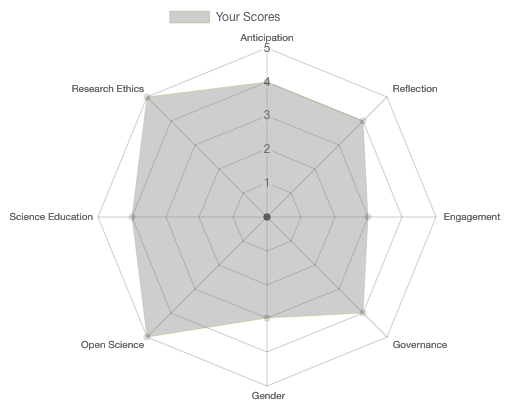
\includegraphics[scale=1.2]{Images/RRI image.png}
    \caption{ORBIT self-assessment visualisation}
    \label{ORBIT RRI}
\end{figure}


\subsection{Anticipate}
It is anticipated that there will be three outputs from this PhD:
1.	An understanding of how proxy data streams can be used to understand and predict well-being
2.	Understanding what data-driven techniques can be used to determine and predict well-being and what techniques are most appropriate.
3.	Understanding how outputs from data-driven models provide value to the various stakeholders involved in the design, provision, or use of digital mental health platforms.

\subsubsection{RRI Approach to Methodologies}
This research will incorporate appropriate data gathering, treatment, and responsible machine learning research methodologies through a meticulous review of current literature. When incorporating data gathered from users, especially digital mental health platforms, which may be highly sensitive, it is crucial to ensure that this data is appropriately anonymised and aggregated. Furthermore, when incorporating data into statistical and machine learning models, it is pertinent that the models being used are appropriate. Hence this research will ensure that a comparison of appropriate methods and frameworks are used for each stage of model development.

\subsubsection{Desirability and Sustainability}
Well-being is a multidimensional construct, and the state of an individual's well-being is ever shifting; this changing state of well-being is difficult to measure and predict. Therefore there is evident desirability for a project such as this to understand and predict well-being trajectories. Combining rich user-based data sources with well-being instruments is a method of understanding and predicting well-being in a nuanced way \parencite{jaidka_estimating_2020}. By using proxy data streams, such as digital mental health platforms and social media data, it is hypothesised that well-being can be understood and predicted; these trajectory outputs could assist various stakeholders involved in the design, provision, or use of digital mental health platforms.

\subsubsection{Stakeholders}
Several stakeholders can provide insight into the scope of the project and enable the appropriate development of research questions and outcomes, and the initial stakeholders are as follows:

•	Digital mental health platform users

•	Various stakeholders involved in the design, provision, or use of digital mental health platforms

•	Machine learning, data science and well-being researchers

•	Adults, children, and young people looking to understand their well-being trajectory

\subsection{Reflect}
Reflection is a vital part of any research project; the key areas of reflection in this research project consist of the inputs used throughout the research and the outputs generated from the research. The reflection of stakeholders, data sources, and machine learning models is vital to understanding the research's wider impact and implications as the project develops.

\subsubsection{Stakeholders, Data and Research Output}
Although a meticulous exploration of stakeholders will be undertaken as part of the initial stages of the research project (see appendix A), there is scope for the project to develop over time. As the direction and focus of the research project shift, it will be necessary to reevaluate the stakeholders of the project; this may be the data sources that are being used or the demographic of the research output. Furthermore, machine learning (ML) is a fast-moving field, reflecting on the ML models that have been used and ensuring the cutting-edge research methods are being implemented while also ensuring the ML techniques are appropriate. 
\subsection{Engage}
\subsubsection{Industry Partner}
A three-month placement with the industry partner early in the first year of the PhD will be undertaken to understand how the research objectives align with the data Kooth can provide throughout the project. This will also enable a more comprehensive understanding of the opportunities provided by the data Kooth can provide as a lens to understand and predict well-being. Furthermore, during the placement and further into the first year of the PhD, landscape mapping projects will be undertaken, such as semi-structured interviews and focus groups with various stakeholders to understand the broader impacts of the research outputs.   
\subsubsection{Digital Mental Health Platform Users}
Users of the platforms are the targets for the outputs of the data-driven models created throughout the research project; therefore, consistent engagement with users through user studies will be crucial for understanding their needs as stakeholders. After the models have been created, an interesting part of the research project will be engaging with users to understand how they perceive the value of model outputs, adding an extra layer of reflection to the research project narrative.
\subsection{Act}
Acting in a research project can have many dimensions. Developing the required technical skills and competencies to undertake and complete the project will involve an exploration of ML techniques and applications, data management competencies, and a rigorous understanding of the landscape of well-being through a psychological lens to understand the wider implications of the research outputs across disciplines. Ensuring flexibility as the research project develops and acting on developments such as new disciplinary techniques.


\printbibliography
\appendix
\section{Appendix Timeline of Planned Activities}
\begin{landscape}
\begin{figure}[h]
    \centering
    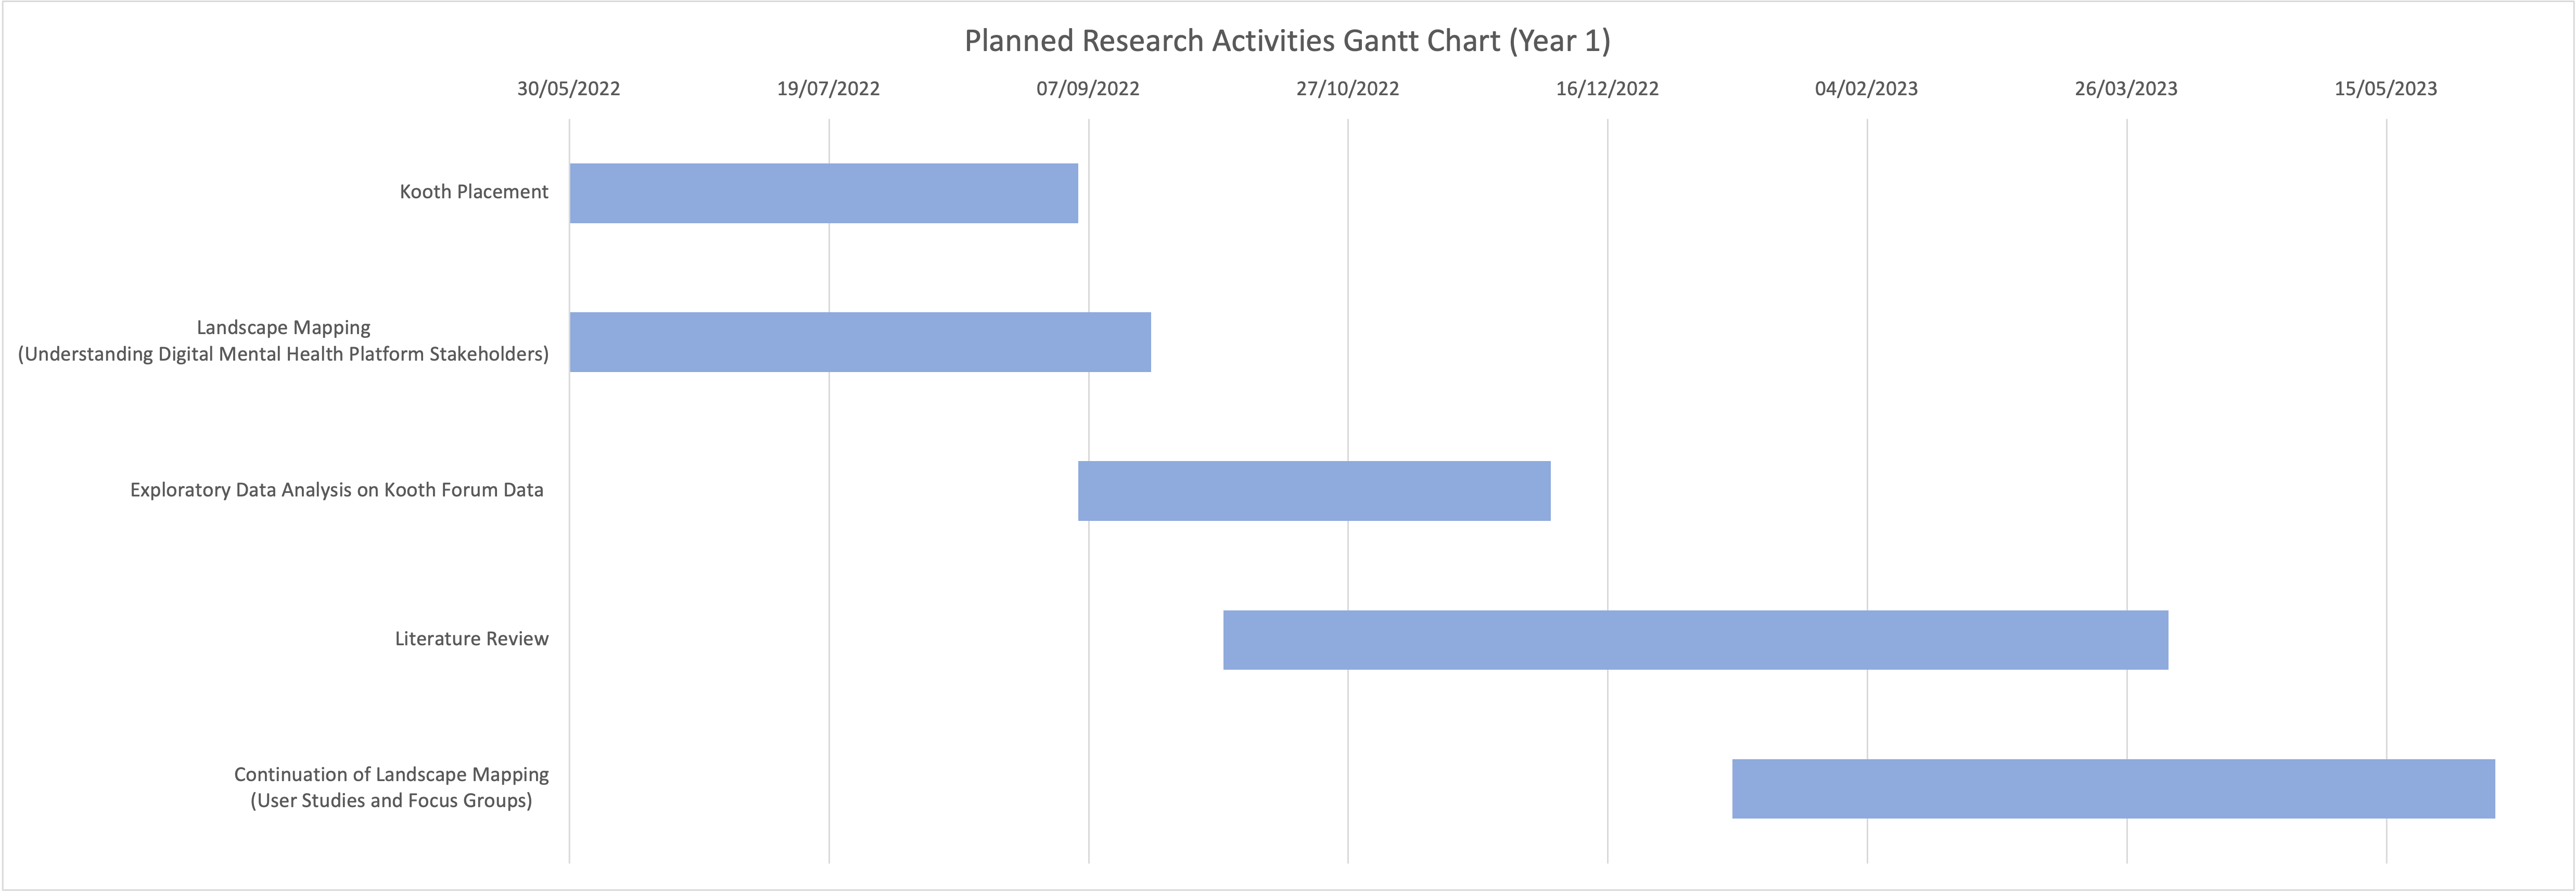
\includegraphics[scale=.6]{Images/Gantt Chart Image.png}
    \caption{Year 1 Gantt Chart}
    \label{Year 1 Gantt Chart}
\end{figure}
\end{landscape}
\subsection*{Year 1}
\centering
 \begin{longtable}{p{0.4\linewidth} | p{0.6\linewidth}}
    \caption{Year 1 Timeline of Planned Activities}
    \hline
      Timeframe  & Description \\ \hline
      30 May 2022 – 05 September 2022 & Kooth Placement/Internship. Understanding the Session Wants and Needs Outcome Measure for service users on Kooth Adult service (Qwell), using Natural Language Processing. This measure is used to understand the wants and needs of a user using the chat service on the Kooth adult service, the chat service is live between the service user and the practitioner. The expected outcomes for this project are an understanding of the techniques of generating topics/themes from mental health platform text data and a research paper relating to item generation using NLP. \\
      \hline
      May 2022 – May 2023& Landscape Mapping Project to understand digital mental health platform stakeholders. This project aims to gain an understanding of the various stakeholders involved the design, provision, or use of digital mental health platforms. This will be achieved through semi-structured interviews with the various stakeholders. This will start with focusing on the platform Kooth, the industry partner for this PhD, to gain an in-depth understanding of their practices and concerns.  Through this investigation, I will be able to frame future PhD research projects to deliver the maximum value to the range of stakeholders and further interviews with those involved in other mental health platforms.\\
      \hline
      Tentative - September 2022 - December 2022 & Exploratory Data Analysis on Kooth Forum Data (10-15 Hours Per Week) This project is an extension of the Safe Space NLP research project in which I will explore if a system could identify and flag up words as potential signs of risk behaviours. Understanding how a system such as this could support Kooth moderators/councillors whilst performing their job, if so, how this could contribute to a priority list of warning signs of harmful behaviours.\\
      \hline
      October 2022 - April 2023 & Conduct a literature review to further understand the current academic literature and incorporate the research into the PhD as an extension to the preliminary literature review conducted in the stage 3 PhD proposal. This will ensure the research addresses an appropriate gap within the multi-disciplinary fields.\\
      \hline
      January 2023 - June 2023&Continuation of Landscape Mapping. Understanding digital mental health platform stakeholders through user surveys and focus groups, specifically for users of digital mental health platforms. This is to understand attitudes and behaviours toward digital mental health platforms and stigma related to the open discussion or lack thereof of mental health/well-being.\\
      \hline
    \end{longtable}
    \label{tab:y1timeline}
\subsection*{Years 2 and 3}    
\centering
    \begin{longtable}{p{1\linewidth}}
    \centering
    \caption{Year 2 and 3 Timeline of Planned Activities}
    
    \hline
      Description \\ 
      \hline
      A review of the different well-being philosophies, certainly an extension of the literature review, enabling the understanding of different use cases for well-being measures; how well-being instruments use language to define well-being - This could play a role in developing a foundational chapter in the PhD thesis based on how measures use language to understand well-being.\\
      \hline
      Exploring and analysing social media and digital mental health data, with scope for additional data sources, as proxy lenses to understand well-being. Exploring questions such as:
      What can the different data sources offer?
      What are the biases, limitations and challenges of using these data sources?\\
      \hline
     Applying data driven techniques to the above proxy lenses to understand what data-driven techniques are most appropriate when attempting to understanding well-being through proxy lenses. This will enable the exploration of potential impacts of understanding and predicting well-being through different data sources.\\
      \hline
    \end{longtable}
    \label{tab:y23timeline}
\end{document}
